\documentclass{standalone}

\usepackage{tikz}
\usetikzlibrary{calc}
\usepackage{color}

\usetikzlibrary{decorations.pathmorphing}
\usetikzlibrary{decorations.pathreplacing,angles,quotes}

\begin{document}

    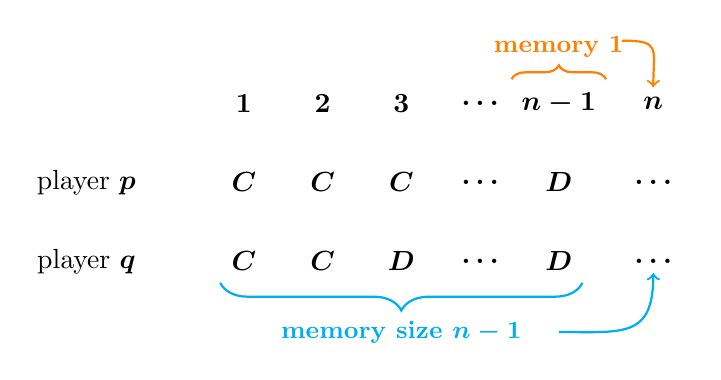
\begin{tikzpicture}

    \tikzstyle{state}=[minimum width=1cm, font=\boldmath];
    

	\node[thick] (0) at (-1, 0) [state] {player $p$};
	\node[thick] (1) at (-1, -1) [state] {player $q$};

	\node[thick] (2) at (1, 1) [state] {$1$};
	\node[thick] (3) at (2, 1) [state] {$2$};
	\node[thick] (4) at (3, 1) [state] {$3$};
	\node[thick] (5) at (4, 1) [state] {$\dots$};
	\node[thick] (6) at (5, 1) [state] {$n - 1$};
	\node[thick] (7) at (6.2, 1) [state] {$n$};

	\node (8) at (1, 0) [state] {$C$};
	\node (9) at (2, 0) [state] {$C$};
	\node (10) at (3, 0) [state] {$C$};
	\node (11) at (4, 0) [state] {$\dots$};
	\node (12) at (5, 0) [state] {$D$};
	\node (13) at (6.2, 0) [state] {$\dots$};

	\node (14) at (1, -1) [state] {$C$};
	\node (15) at (2, -1) [state] {$C$};
	\node (16) at (3, -1) [state] {$D$};
	\node (17) at (4, -1) [state] {$\dots$};
	\node (18) at (5, -1) [state] {$D$};
	\node (19) at (6.2, -1) [state] {$\dots$};

	\draw[decoration={brace, raise=6pt, amplitude=5pt}, decorate, orange, thick] 
	(4.4, 1.1) -- node[above=10pt] {\textcolor{orange}{\textbf{\small{memory \boldmath$1$}}}} (5.6, 1.1);

	\draw[decoration={brace, mirror, raise=5pt, amplitude=10pt}, decorate, cyan, thick] 
	(0.7, -1.1) -- node[below=15pt] {\textcolor{cyan}{\textbf{\small{memory size \boldmath$n -1$}}}} (5.3, -1.1);
	
	\coordinate (s)  at (5.8, 1.8);

	\draw[orange, looseness=1.8] (s) edge[out=0, in=90, ->, thick] (7);

	\coordinate (n)  at (5, -1.9);

	\draw[cyan, looseness=1.5] (n) edge[out=0, in=-90, ->, thick] (19);

	\end{tikzpicture}

\end{document}